\section{TỔNG QUAN VỀ ĐIỆN TOÁN ĐÁM MÂY}
\subsection{Khái niệm và đặc điểm của điện toán đám mây}
\subsubsection{Lịch sử ra đời của điện toán đám mây}
Khái niệm điện toán đám mây ra đời từ những năm 1950 khi máy chủ tính toán quy mô lớn (large-scale mainframe computers) được triển khai tại một số cơ sở giáo dục và tập đoàn lớn. Tài nguyên tính toán của các hệ thống máy chủ được truy cập từ các máy khách cuối (thin clients, terminal computers), từ đó khai sinh khái niệm “chia sẻ thời gian” (time-sharing) đặc tả việc cho phép nhiều người sử dụng cùng chia sẻ đồng thời một tài nguyên tính toán chung.

Trong những năm 1960 – 1990, xuất hiện luồng tư tưởng coi máy tính hay tài nguyên công nghệ thông tin có thể được tổ chức như hạ tầng dịch vụ công cộng (public utility). Điện toán đám mây hiện tại cung cấp tài nguyên tính toán dưới dạng dịch vụ và tạo cảm giác cho người dùng về một nguồn cung ứng là vô tận. Đặc tính này có thể so sánh tới các đặc tính của ngành công nghiệp tiêu dùng dịch vụ công cộng như điện và nước. Khi sử dụng điện hay nước, người dùng không cần quan tâm tới tài nguyên đến từ đâu, được xử lý, phân phối như thế nào, họ chỉ việc sử dụng dịch vụ và trả tiền cho nhà cung cấp theo lượng tiêu dùng của mình.

Những năm 1990, các công ty viễn thông từ chỗ cung ứng kênh truyền dữ liệu điểm tới điểm (point-to-point data circuits) riêng biệt đã bắt đầu cung ứng các dịch vụ mạng riêng ảo với giá thấp. Thay đổi này tạo tiền đề để các công ty viễn thông sử dụng hạ tầng băng thông mạng hiệu quả hơn. Điện toán đám mây mở rộng khái niệm chia sẻ băng thông mạng này qua việc cho phép chia sẻ cả tài nguyên máy chủ vật lý bằng việc cung cấp các máy chủ ảo.

Amazon cung cấp nền tảng Amazon Web Services (AWS) vào năm 2006, đánh dấu việc thương mại hóa điện toán đám mây. Từ đầu năm 2008, Eucalyptus được giới thiệu là nền tảng điện toán đám mây mã nguồn mở đầu tiên, tương thích với API của AWS. Tính tới thời điểm hiện tại, có rất nhiều các sản phẩm điện toán đám mây được đưa ra như Google App Engine, Microsoft Azure, Nimbus,..

\subsubsection{Khái niệm điện toán đám mây}
Điện toán đám mây là một mô hình cho phép thuận tiện, truy cập mạng theo yêu cầu đến một nơi chứa các nguồn tài nguyên tính toán có thể chia sẻ và cấu hình được (ví dụ: mạng, máy chủ, lưu trữ, ứng dụng và dịch vụ), có thể được cung cấp và phát hành nhanh chóng với nỗ lực quản lý hoặc tương tác với nhà cung cấp tối thiểu \cite{hostvn_cloud_computing}.
\begin{figure}[H] % cần gói float nếu muốn fix vị trí
    \centering
    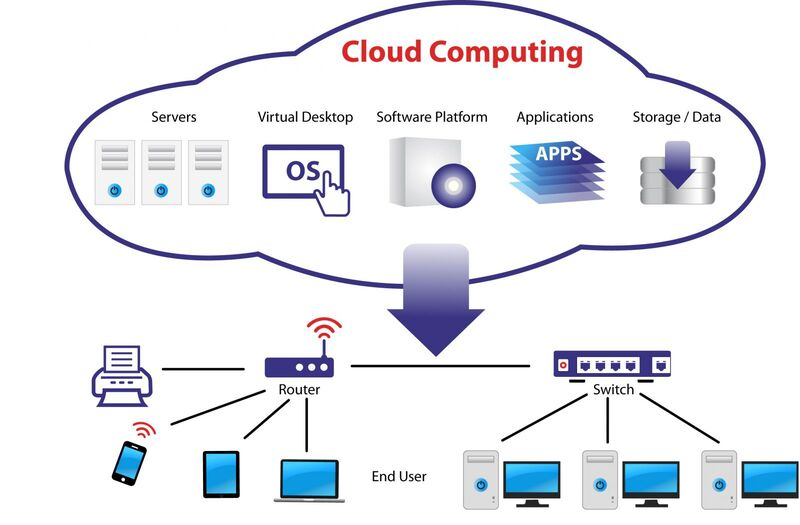
\includegraphics[width=0.7\textwidth]{Tong_quan_DTDM/dien-toan-dam-may-la-gi.jpg}
    \caption{Kiến trúc mô hình điện toán đám mây}
    \label{fig:cloud_intro}
\end{figure}

Điện toán đám mây (cloud) có thể được sử dụng cho nhiều mục đích khác nhau: machine learning, data analysis, storage \& backup, streaming media content và hơn thế nữa. Một ví dụ thực tế, tất cả các chương trình và phim bạn xem trên Netflix thực sự được lưu trữ trên đám mây. Ngoài ra, đám mây có thể có lợi cho việc tạo và thử nghiệm các ứng dụng, tự động hóa việc phân phối phần mềm và lưu trữ v.v..\cite{aws_cloud_file_storage}.

Các nhà cung cấp dịch vụ đám mây có các trung tâm dữ liệu khổng lồ chứa hàng trăm máy chủ, hệ thống lưu trữ và các thành phần quan trọng dành cho nhiều loại doanh nghiệp khác nhau. Các trung tâm dữ liệu này nằm ở những vị trí an toàn và lưu trữ một lượng lớn dữ liệu. Người dùng kết nối với các trung tâm dữ liệu này để thu thập dữ liệu hoặc sử dụng nó khi được yêu cầu. Người dùng có thể tận dụng các dịch vụ khác nhau; ví dụ: nếu bạn muốn có thông báo mỗi khi ai đó gửi cho bạn một văn bản hoặc email, các dịch vụ đám mây có thể giúp bạn làm điều này. Phần tốt nhất về nền tảng đám mây là bạn chỉ trả tiền cho các dịch vụ mà bạn sử dụng và không có chi phí trả trước.

\subsubsection{Đặc điểm của điện toán đám mây}
Định nghĩa của US NIST chứa đựng kiến trúc, an ninh và chiến lược triển khai của đám mây với năm đặc tính cốt lõi của điện toán đám mây là:

\begin{myitem}
\item Tự phục vụ theo yêu cầu (on-demand self-service): Khách hàng với nhu cầu tức thời tại những thời điểm thời gian xác định có thể sử dụng các tài nguyên tính toán (như thời gian CPU, không gian lưu trữ mạng, sử dụng phần mềm,...) một cách tự động, không cần tương tác với con người để cấp phát.

\item Sự truy cập mạng rộng rãi (broad network access): Những tài nguyên tính toán này được phân phối qua mạng Internet và được các ứng dụng client khác nhau sử dụng với những nền tảng không đồng nhất (như máy tính, điện thoại di động, PDA).

\item Tập trung tài nguyên: Những tài nguyên tính toán của nhà cung cấp dịch vụ đám mây được tập trung với mục đích phục vụ đa khách hàng sử dụng mô hình ảo hóa với những tài nguyên vật lý và tài nguyên ảo được cấp phát động theo yêu cầu. Động lực của việc xây dựng một mô hình tập trung tài nguyên tính toán nằm trong hai yếu tố quan trọng: tính quy mô và tính chuyên biệt. Kết quả của mô hình tập trung tài nguyên là những tài nguyên vật lý trở nên trong suốt với người sử dụng. Ví dụ, người sử dụng không được biết vị trí lưu trữ cơ sở dữ liệu của họ trong đám mây.

\item Tính mềm dẻo: Đối với người sử dụng, các tài nguyên tính toán được cung cấp tức thời hơn là liên tục, được cung cấp theo nhu cầu để mở rộng hoặc tiết giảm không hạn định tại bất kỳ thời điểm nào.

\item Dịch vụ đo lường: Hệ thống điện toán tự động kiểm soát và tối ưu hóa việc sử dụng nguồn lực bằng cách áp dụng khả năng đo lường ở các mức độ trừu tượng phù hợp với từng loại dịch vụ. Việc sử dụng tài nguyên có thể được kiểm soát, giám sát và báo cáo, cung cấp thông tin minh bạch về việc sử dụng dịch vụ đối với cả nhà cung cấp và khách hàng.
\end{myitem}

\begin{figure}[H] % cần gói float nếu muốn fix vị trí
    \centering
    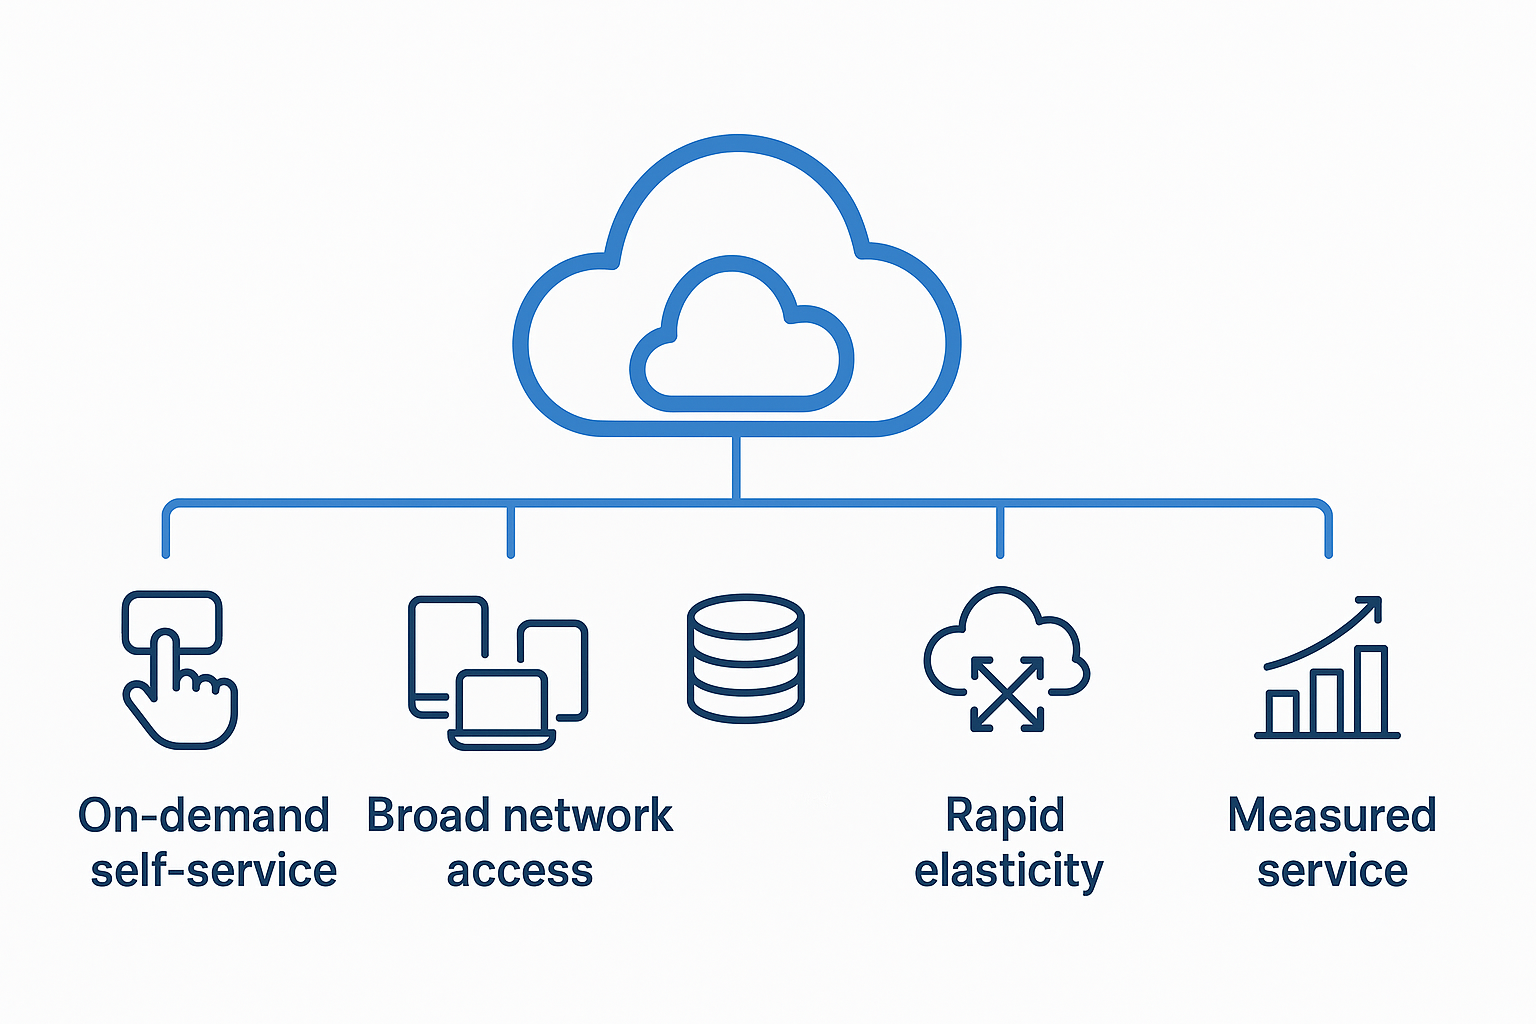
\includegraphics[width=0.7\textwidth]{Tong_quan_DTDM/Dac_diem_DTDM.png}
    \caption{Đặc điểm của điện toán đám mây}
    \label{fig:cloud_intro}
\end{figure}

\subsection{Ưu điểm và nhược điểm của hệ thống điện toán đám mây}
\begin{myitem}
\item Ưu điểm của dịch vụ lưu trữ đám mây:
  \begin{mysubitem}
  \item Tiết kiệm chi phí: Không cần đầu tư vào phần cứng lưu trữ vật lý, người dùng chỉ trả tiền cho dung lượng lưu trữ và dịch vụ mà họ thực sự sử dụng.
  \item Khả năng mở rộng linh hoạt: Dung lượng lưu trữ có thể dễ dàng tăng hoặc giảm theo nhu cầu mà không cần thay đổi cơ sở hạ tầng.
  \item Truy cập từ xa: Dữ liệu có thể được truy cập từ bất kỳ đâu qua internet, thuận tiện cho việc làm việc từ xa và chia sẻ tài liệu.
  \item Sao lưu và phục hồi dữ liệu: Nhiều dịch vụ lưu trữ đám mây cung cấp tính năng sao lưu tự động và phục hồi dữ liệu, giúp bảo vệ dữ liệu khỏi mất mát hoặc sự cố.
  \item Bảo mật và mã hóa: Các nhà cung cấp dịch vụ lưu trữ đám mây thường áp dụng các biện pháp bảo mật và mã hóa dữ liệu, giúp bảo vệ thông tin khỏi truy cập trái phép.
  \end{mysubitem}

\item Nhược điểm của dịch vụ lưu trữ đám mây:
  \begin{mysubitem}
  \item Vấn đề bảo mật và quyền riêng tư: Dữ liệu được lưu trữ trên máy chủ của bên thứ ba có thể gặp rủi ro về bảo mật và quyền riêng tư, đặc biệt nếu nhà cung cấp không có biện pháp bảo vệ đủ mạnh.
  \item Phụ thuộc vào kết nối internet: Truy cập và quản lý dữ liệu phụ thuộc vào kết nối internet, có thể gây khó khăn nếu kết nối không ổn định hoặc không có kết nối.
  \item Chi phí phát sinh: Mặc dù chi phí ban đầu thấp, nhưng việc lưu trữ dữ liệu lớn hoặc nhiều người dùng có thể dẫn đến chi phí phát sinh không lường trước được.
  \item Khó khăn trong quản lý dữ liệu lớn: Quản lý và tổ chức dữ liệu lớn có thể trở nên phức tạp, đặc biệt nếu không có các công cụ quản lý dữ liệu hiệu quả.
  \item Khả năng phụ thuộc vào nhà cung cấp: Doanh nghiệp có thể gặp khó khăn trong việc di chuyển dữ liệu hoặc ứng dụng nếu muốn chuyển sang nhà cung cấp khác hoặc đưa trở lại quản lý nội bộ.
  \end{mysubitem}
\end{myitem}

\subsection{Sơ lược các công nghệ ứng dụng trong điện toán đám mây}
\subsubsection{Công nghệ ảo hoá}
Công nghệ ảo hóa (virtualization) là công nghệ quan trọng nhất ứng dụng trong điện toán đám mây. Công nghệ ảo hóa là công nghệ cho phép tạo ra các thực thể ảo có tính năng tương đương như các thực thể vật lý, ví dụ như thiết bị lưu trữ, bộ vi xử lý,… Ảo hóa phần cứng (hardware virtualization) tham chiếu tới việc tạo ra các máy ảo (virtual machine) mà hoạt động với hệ điều hành được cài đặt như một máy tính vật lý thực. Ví dụ, một máy ảo chạy hệ điều hành Ubuntu có thể được tạo ra trên một máy tính thực cài hệ điều hành Windows.


Điều này được thể hiện qua việc có thể khởi tạo nhiều máy ảo với năng lực tính toán và năng lực lưu trữ bé hơn trên duy nhất một máy chủ vật lý. Máy chủ vật lý được gọi là host machine còn máy ảo (virtual machine) được gọi là máy khách (guest machine). Khái niệm "host" và "guest" được sử dụng để phân biệt phần mềm chạy trên máy tính vật lý hay phần mềm chạy trên máy ảo. Phần mềm hay firmware tạo máy ảo được gọi là hypervisor hay virtual machine manager.

Thông thường việc đầu tư cho một trung tâm công nghệ thông tin rất tốn kém. Chi phí mua các máy chủ cấu hình mạng và các phần mềm bản quyền rất là đắt. Vậy nên việc ảo hóa trở thành nhu cầu cần thiết cho bất kỳ doanh nghiệp nào. Bởi thay vì mua 10 máy chủ cho 10 ứng dụng thì chỉ cần mua một hai máy chủ có hỗ trợ ảo hóa vẫn có thể chạy tốt cả 10 ứng dụng. Điều này cho thấy sự khác biệt giữa hệ thống ảo hóa và không ảo hóa. Ngoài ra việc ảo hóa còn có các lợi ích sau:

\begin{myitem}
\item Quản lý đơn giản;

\item Tiển khai nhanh;

\item Phục hồi và lưu trữ hệ thống nhanh;

\item Cân bằng tải và phân phối tài nguyên linh hoạt;

\item Tiết kiệm chi phí;

\item Ảo hóa góp phần tăng cường tính liên tục, hạn chế ngắt quãng.
\end{myitem}

\subsubsection{Công nghệ tự động hóa giám sát điều phối tài nguyên (automation, dynamic dynamic orchestration)}
Công nghệ giám sát điều phối tài nguyên động là nền tảng để điện toán đám mây thực hiện cam kết chất lượng cung cấp dịch vụ điện toán. Với công nghệ điều phối tài nguyên động, việc lắp đặt thêm hay giảm bớt các tài nguyên máy chủ vật lý hoặc máy chủ lưu trữ dữ liệu được thực hiện tự động để hệ thống điện toán luôn đáp ứng được giao kèo trong hợp đồng dịch vụ đã ký với bên người sử dụng.

\subsubsection{Công nghệ tính toán phân tán, hệ phân tán}
Điện toán đám mây là một dạng hệ phân tán xuất phát từ yêu cầu cung ứng dịch vụ cho lượng người sử dụng khổng lồ. Tài nguyên tính toán của điện toán đám mây là tổng thể kết hợp của hạ tầng mạng và hàng nghìn máy chủ vật lý phân tán trên một hay nhiều trung tâm dữ liệu số (data centers).

\subsubsection{Công nghệ Web 2.0}
Web 2.0 là nền tảng công nghệ phát triển các sản phẩm ứng dụng hướng dịch vụ trên nền điện toán đám mây. Công nghệ Web 2.0 phát triển cho phép phát triển giao diện ứng dụng web dễ dàng và nhanh chóng và trên nhiều thiết bị giao diện khác nhau. Web 2.0 phát triển làm xóa đi khoảng cách về thiết kế giao diện giữa ứng dụng máy tính thông thường và ứng dụng trên nền web, cho phép chuyển hóa ứng dụng qua dịch vụ trên nền điện toán đám mây mà không ảnh hưởng đến thói quen người sử dụng.

\subsection{Một số đám mây được triển khai phổ biến hiện nay}
Hiện nay, các đám mây được chia thành hai nhóm:

\begin{myitem}
\item Thứ nhất, Ba “Hyperscaler” hàng đầu (Thị phần toàn cầu lớn nhất):
  \begin{mysubitem}
  \item Amazon Web Services (AWS): Dẫn đầu thị trường với khoảng 29--32\% thị phần toàn cầu quý 1 năm 2025, AWS sở hữu hệ sinh thái dịch vụ phong phú (hơn 200 dịch vụ), vùng hoạt động rộng khắp toàn cầu và năng lực hỗ trợ AI nổi bật.
  
  \item Microsoft Azure: Xếp thứ hai, chiếm khoảng 22 - 24\% thị phần, Azure mạnh ở mảng tích hợp với hệ sinh thái Microsoft (365, Active Directory\ldots), hỗ trợ hybrid cloud tốt (Azure Arc, Stack) và được doanh nghiệp lớn ưa chuộng.
  
  \item Google Cloud Platform (GCP): Đứng thứ ba với khoảng 12\% thị phần toàn cầu, GCP nổi bật về năng lực trong AI/ML, phân tích dữ liệu (BigQuery, Vertex AI), container hoá (Kubernetes), và được đánh giá cao bởi các startup \& tech-savvy teams.
  \end{mysubitem}

\begin{figure}[H] % cần gói float nếu muốn fix vị trí
    \centering
    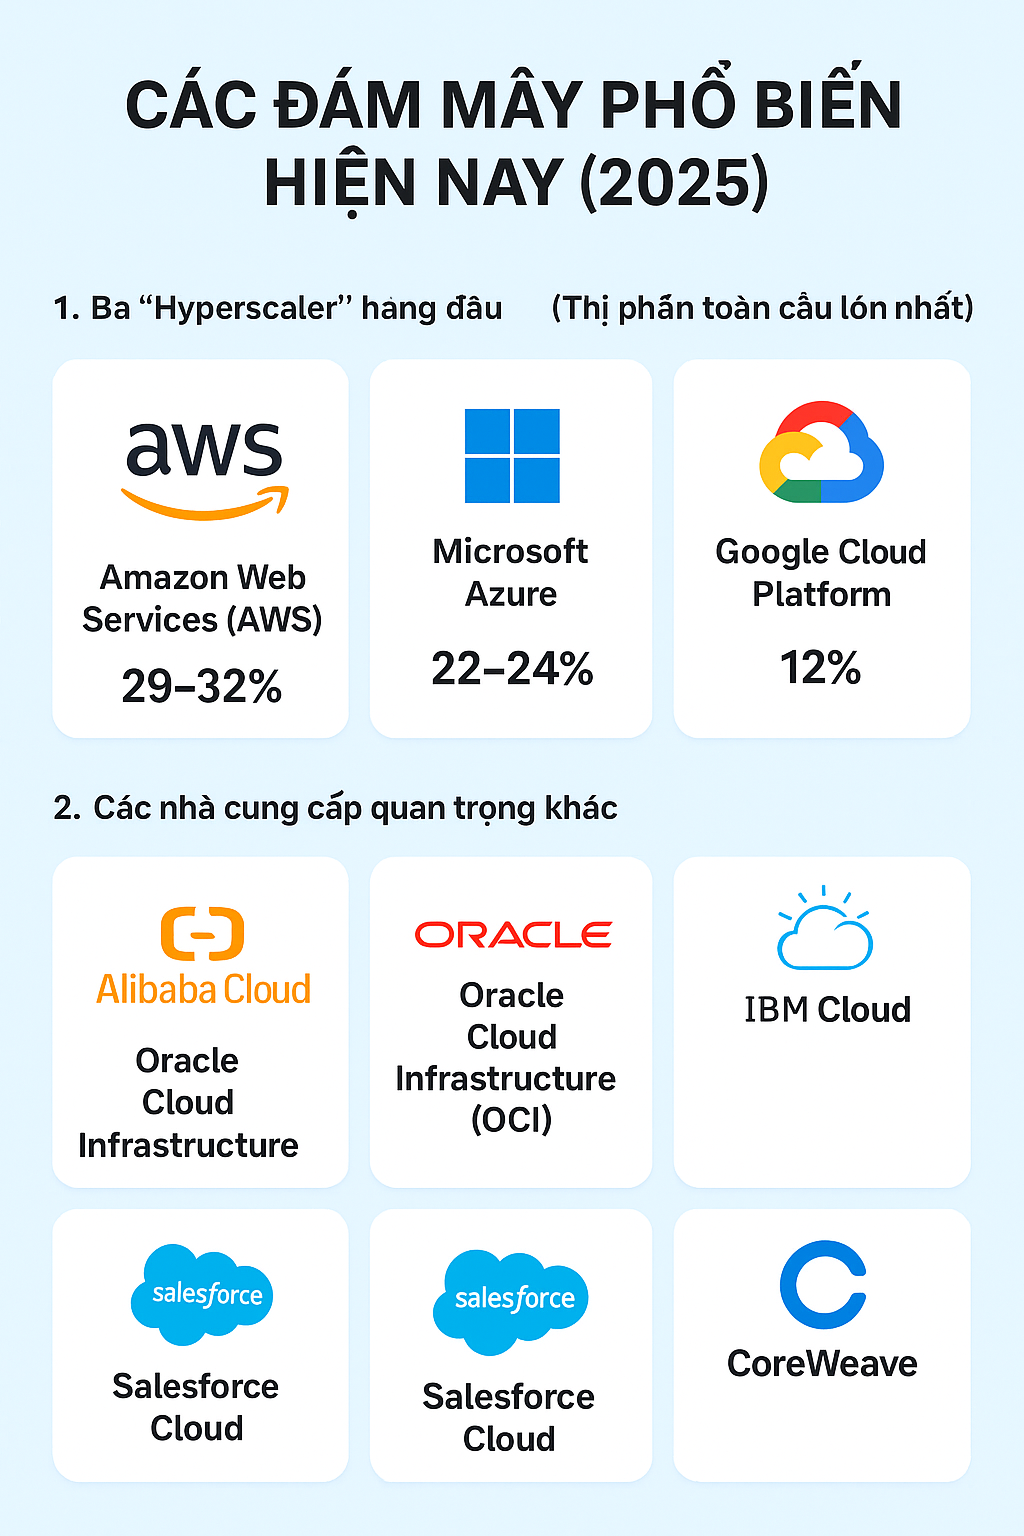
\includegraphics[width=0.7\textwidth]{Tong_quan_DTDM/Cac_dam_may_pho_bien.png}
    \caption{Các đám mây được triển khai phổ biến hiện nay}
    \label{fig:cloud_intro}
\end{figure}


\item Thứ hai, Các nhà cung cấp quan trọng khác:
  \begin{mysubitem}
  \item Alibaba Cloud - Khoảng 4\% thị phần toàn cầu, đặc biệt mạnh ở khu vực Châu Á -- Thái Bình Dương.
  
  \item Oracle Cloud Infrastructure (OCI) -- Chiếm 3\% thị phần, phát triển nhanh với nền tảng tối ưu hiệu năng cao, đặc biệt cho các hệ thống Oracle truyền thống.
  
  \item Tencent Cloud -- Khoảng 2\% thị phần toàn cầu, nhưng là nhà cung cấp lớn thứ ba tại Trung Quốc với khoảng 15\% nội địa. Phát triển mạnh ở Đông Nam Á.
  
  \item Các nhà cung cấp khác như OVHcloud, DigitalOcean, Linode, Kamatera\ldots\ nổi bật ở mảng nhỏ và vừa, developer-friendly, hoặc phục vụ nhu cầu địa phương/chi phí thấp.
  \end{mysubitem}
\end{myitem}

\subsection{Các loại hình dịch vụ}
Điện toán đám mây có ba mô hình cung cấp dịch vụ, tùy theo các đối tượng khách hàng như sau \cite{vngcloud_iaas_paas_saas}:

\begin{myitem}
\item Infrastructure as a Service – Dịch vụ hạ tầng

\item Platform as a Service – Dịch vụ nền tảng

\item Software as a Service – Dịch vụ phần mềm

\end{myitem}

\begin{figure}[H] % cần gói float nếu muốn fix vị trí
    \centering
    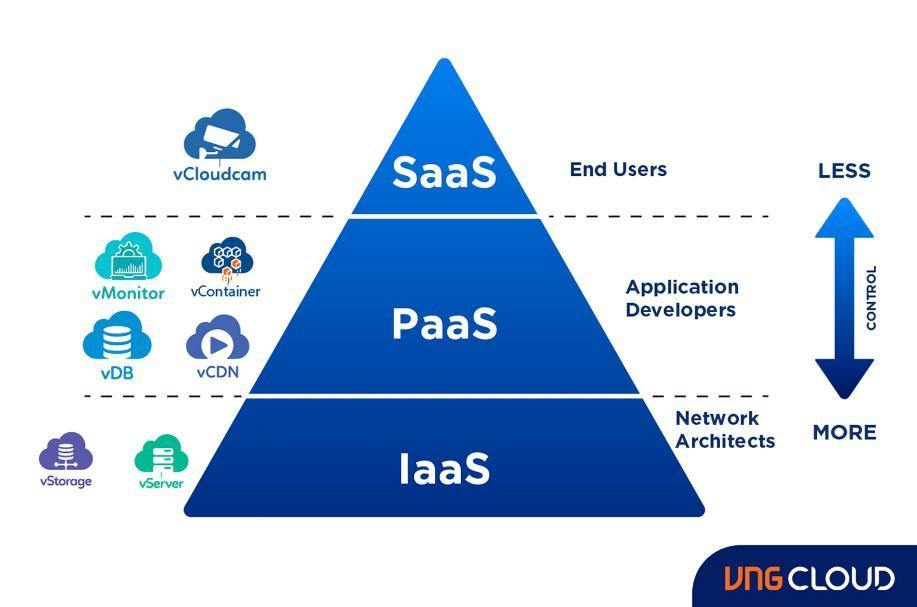
\includegraphics[width=0.7\textwidth]{Tong_quan_DTDM/Cac_loai_hinh_dich_vu.jpg}
    \caption{Mỗi mô hình cung cấp các mức độ quản lý và chức năng khác nhau, cho
phép doanh nghiệp lựa chọn mô hình phù hợp nhất với nhu cầu}
    \label{fig:cloud_intro}
\end{figure}

\subsubsection{Infrastructure as a Service (IaaS)}
\begin{myitem}
  \item \textbf{Định nghĩa:} Cung cấp cơ sở hạ tầng công nghệ thông tin như máy chủ, lưu trữ và mạng qua đám mây.

  \item \textbf{Quyền kiểm soát:} Người dùng có toàn quyền quản lý cơ sở hạ tầng, hệ điều hành, ứng dụng.

  \item \textbf{Đối tượng sử dụng:} Doanh nghiệp cần kiểm soát và tùy chỉnh hạ tầng theo nhu cầu riêng.

  \item \textbf{Ưu điểm:}
    \begin{mysubitem}
      \item Doanh nghiệp có thể thiết kế, điều chỉnh cơ sở hạ tầng theo nhu cầu.
      \item Tiết kiệm chi phí mua phần cứng.
      \item Dễ dàng mở rộng hoặc thu hẹp tài nguyên theo sự phát triển của doanh nghiệp.
      \item Người dùng có quyền quản lý toàn bộ hệ điều hành và ứng dụng.
    \end{mysubitem}

  \item \textbf{Nhược điểm:} Yêu cầu có chuyên môn kỹ thuật, có đội ngũ công nghệ thông tin để quản lý và bảo trì.
\end{myitem}

\begin{figure}[H] % cần gói float nếu muốn fix vị trí
    \centering
    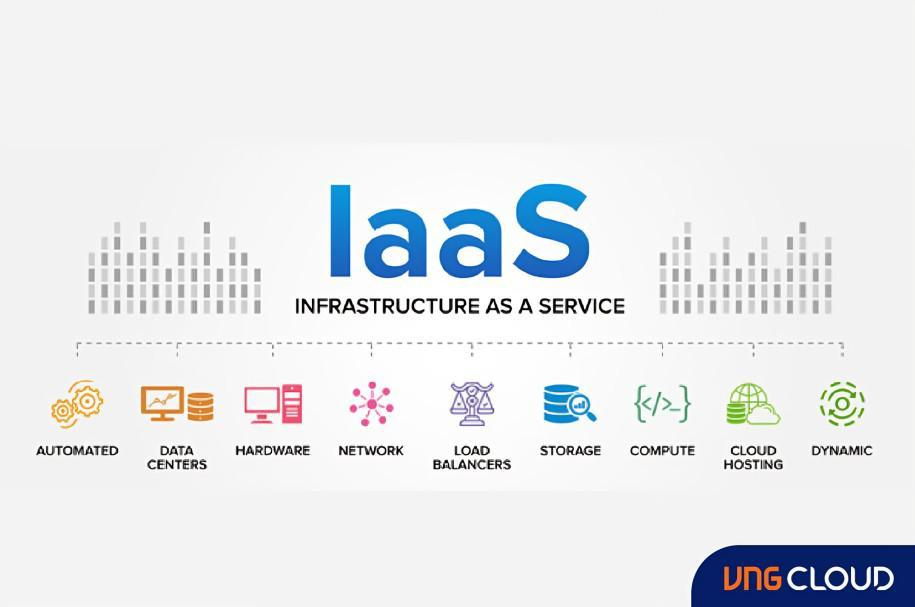
\includegraphics[width=0.7\textwidth]{Tong_quan_DTDM/IaaS.jpg}
    \caption{Nhà cung cấp IaaS có trách nhiệm trong việc bảo mật cơ sở hạ tầng
dành riêng cho ứng dụng điện toán đám mây}
    \label{fig:cloud_intro}
\end{figure}

\subsubsection{Platform as a Service (PaaS)}
\begin{myitem}
  \item \textbf{Định nghĩa:} Cung cấp nền tảng phát triển và triển khai ứng dụng mà không cần quản lý hạ tầng.

  \item \textbf{Quyền kiểm soát:} Người dùng quản lý ứng dụng nhưng không kiểm soát cơ sở hạ tầng.

  \item \textbf{Đối tượng sử dụng:} Các nhà phát triển muốn tập trung vào viết mã mà không lo về cơ sở hạ tầng.

  \item \textbf{Ưu điểm:}
    \begin{mysubitem}
      \item Không cần bảo trì và cập nhật hệ thống máy chủ.
      \item Nhà phát triển có thể tập trung vào viết mã và ứng dụng.
      \item PaaS cung cấp các công cụ sẵn có giúp giảm thời gian phát triển ứng dụng.
      \item Tạo điều kiện cho việc hợp tác giữa các thành viên nhóm phát triển.
    \end{mysubitem}

  \item \textbf{Nhược điểm:} Khả năng kiểm soát cơ sở hạ tầng bị hạn chế, phải phụ thuộc vào nhà cung cấp.
\end{myitem}

\begin{figure}[H] % cần gói float nếu muốn fix vị trí
    \centering
    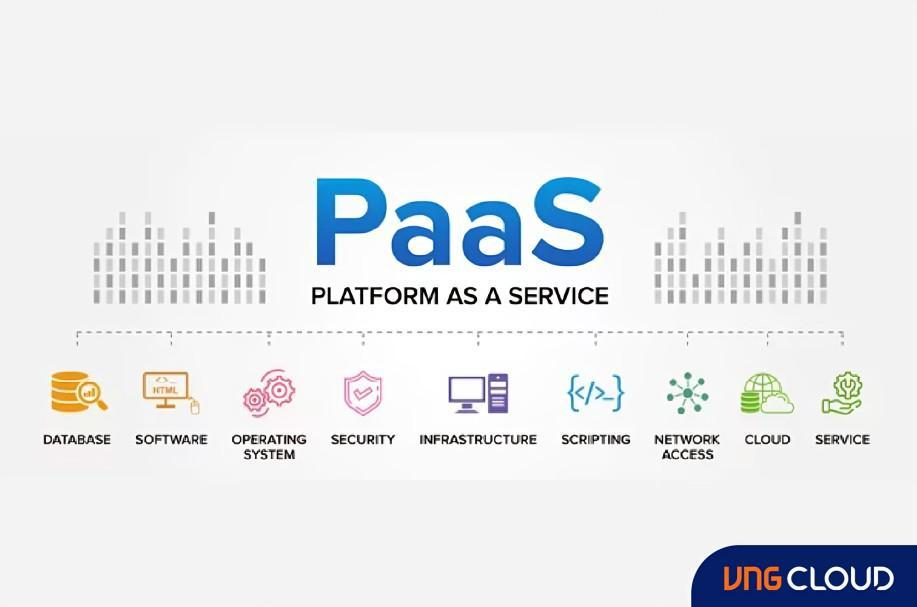
\includegraphics[width=0.9\textwidth]{Tong_quan_DTDM/PaaS.jpg}
    \caption{PaaS là mô hình dịch vụ điện toán đám mây trong đó nhà cung cấp bên
thứ ba cung cấp các công cụ phần cứng và phần mềm cho người dùng thông qua
Internet}
    \label{fig:cloud_intro}
\end{figure}

\subsubsection{Software as a Service (SaaS)}
\begin{myitem}
  \item \textbf{Định nghĩa:} Cung cấp phần mềm hoàn chỉnh thông qua internet mà không cần cài đặt.

  \item \textbf{Quyền kiểm soát:} Người dùng chỉ sử dụng phần mềm, nhà cung cấp quản lý toàn bộ.

  \item \textbf{Đối tượng sử dụng:} Người dùng cuối (End User) hoặc doanh nghiệp cần phần mềm để sử dụng ngay.

  \item \textbf{Ưu điểm:}
    \begin{mysubitem}
      \item Phần mềm có sẵn để sử dụng ngay qua internet mà không cần cài đặt.
      \item Nhà cung cấp dịch vụ chịu trách nhiệm quản lý, cập nhật và bảo mật phần mềm.
      \item Không cần chi phí phát triển hoặc quản lý phần mềm.
      \item Người dùng có thể sử dụng phần mềm với bất kỳ thiết bị nào có kết nối internet.
    \end{mysubitem}

  \item \textbf{Nhược điểm:} Khả năng tùy chỉnh hạn chế, phụ thuộc vào nhà cung cấp dịch vụ.
\end{myitem}

\begin{figure}[H] % cần gói float nếu muốn fix vị trí
    \centering
    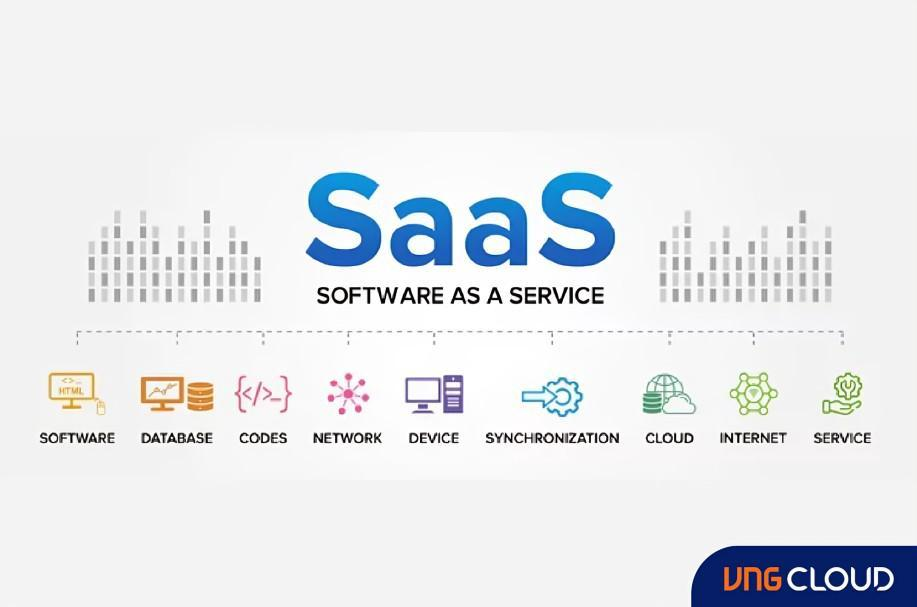
\includegraphics[width=0.7\textwidth]{Tong_quan_DTDM/SaaS.jpg}
    \caption{SaaS cung cấp sự lựa chọn về phần mềm và bảo trì của bên thứ
ba toàn diện nhất}
    \label{fig:cloud_intro}
\end{figure}

\subsection{Xử lý dữ liệu phân tán}
\begin{myitem}
  \item NFS (Network File System): Cho phép chia sẻ tập tin cho nhiều người dùng trên cùng mạng và người dùng có thể thao tác như với tập tin trên chính đĩa cứng của mình.

  \item AFS (Andrew File System): Hệ thống tập tin phân tán nhằm mục đích chia sẻ tập tin cho một lượng lớn người dùng mạng. So với NFS, AFS có tính khả mở cao hơn, đáp ứng được số lượng người dùng lớn hơn nhờ cơ chế sau:
    \begin{mysubitem}
      \item Khi truy cập tập tin, toàn bộ tập tin sẽ được sao chép về phía máy người sử dụng và các thao tác đọc/ghi được thực hiện trên tập tin đó.
      \item Khi tập tin được đóng, nội dung tập tin sẽ được cập nhật về phía máy chủ lưu trữ. Do đó, quá trình đọc/ghi đồng thời là trong suốt đối với từng người dùng, nhưng tính nhất quán của tập tin không được đảm bảo.
    \end{mysubitem}

  \item GFS (Google File System): Hệ thống tệp phân tán của Google, được thiết kế để lưu trữ và xử lý dữ liệu lớn, tối ưu cho các tác vụ đọc/ghi dữ liệu lớn và hỗ trợ độ bền cao.

\begin{figure}[H] % cần gói float nếu muốn fix vị trí
    \centering
    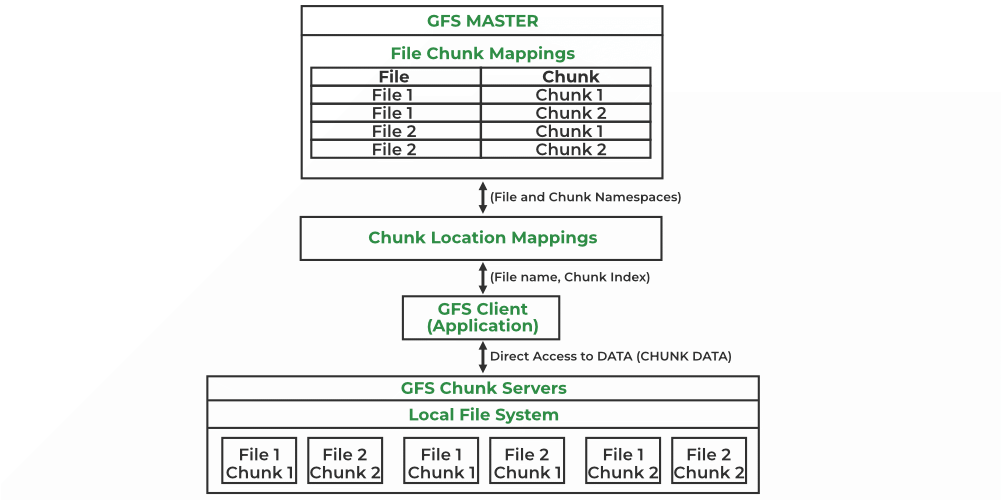
\includegraphics[width=0.9\textwidth]{Tong_quan_DTDM/GFS.png}
    \caption{Google File System}
    \label{fig:cloud_intro}
\end{figure}

  \item HDFS (Hadoop Distributed File System): Hệ thống tệp phân tán dùng trong Apache Hadoop, cho phép lưu trữ và xử lý dữ liệu lớn trên nhiều máy tính. HDFS được tối ưu cho xử lý dữ liệu phân tán, chịu lỗi tốt và có khả năng mở rộng.

  \item RDBMS (Relational Database Management System): Hệ quản trị cơ sở dữ liệu quan hệ, sử dụng bảng để lưu trữ dữ liệu và hỗ trợ các truy vấn SQL để xử lý dữ liệu.  
  Ví dụ: MySQL, PostgreSQL.

  \item NoSQL: Cơ sở dữ liệu phi quan hệ, không sử dụng bảng và SQL, thích hợp cho ứng dụng yêu cầu xử lý dữ liệu phi cấu trúc và có khả năng mở rộng cao.  
  Ví dụ: MongoDB, Cassandra.
\end{myitem}

\subsection{Mô hình triển khai hệ thống điện toán đám mây}
\begin{myitem}
  \item Public Cloud (Đám mây “công cộng”)  

  \hspace*{1cm}Public Cloud là mô hình đám mây do bên thứ ba (các nhà cung cấp dịch vụ đám mây như AWS, Microsoft Azure, Google Cloud, IBM Cloud, v.v.) cung cấp và quản lý. Các dịch vụ này được triển khai trên hạ tầng nằm ngoài tường lửa của doanh nghiệp và được chia sẻ cho nhiều người dùng hoặc tổ chức khác nhau. Người dùng sẽ đăng ký và trả phí sử dụng theo chính sách giá của nhà cung cấp, thường dựa trên mức tiêu thụ tài nguyên (pay-as-you-go) \cite{aws_public_vs_private_cloud}..  

  \hspace*{1cm}Ưu điểm của mô hình này là tính linh hoạt, khả năng mở rộng gần như vô hạn, tiết kiệm chi phí đầu tư ban đầu và dễ dàng tiếp cận. Đây là mô hình phổ biến nhất hiện nay, phù hợp với các cá nhân, doanh nghiệp vừa và nhỏ, hoặc các tổ chức cần triển khai dịch vụ nhanh chóng mà không muốn đầu tư nhiều vào cơ sở hạ tầng.  

  \item Private Cloud (Đám mây “doanh nghiệp”) 

  \hspace*{1cm}Private Cloud được xây dựng và triển khai riêng biệt cho một doanh nghiệp hoặc tổ chức, thường nằm trong hệ thống mạng nội bộ và được bảo vệ bởi tường lửa. Việc quản lý và vận hành có thể do chính doanh nghiệp thực hiện hoặc thuê đối tác chuyên trách \cite{aws_public_vs_private_cloud}.  

  \hspace*{1cm}Điểm mạnh của mô hình này là tính bảo mật cao, khả năng kiểm soát toàn diện và khả năng tùy chỉnh hạ tầng theo nhu cầu riêng. Private Cloud phù hợp với các tổ chức lớn, cơ quan chính phủ, ngân hàng, tài chính, hoặc những đơn vị có yêu cầu nghiêm ngặt về bảo mật dữ liệu. Tuy nhiên, chi phí đầu tư và bảo trì hệ thống thường cao hơn so với Public Cloud.  

  \item Hybrid Cloud (Đám mây “lai”)  

  \hspace*{1cm}Hybrid Cloud là sự kết hợp giữa Public Cloud và Private Cloud, tạo nên một mô hình linh hoạt, giúp doanh nghiệp tận dụng được lợi thế của cả hai. Doanh nghiệp có thể triển khai các dịch vụ quan trọng, yêu cầu bảo mật cao trên Private Cloud, trong khi tận dụng Public Cloud để mở rộng năng lực xử lý hoặc lưu trữ khi có nhu cầu đột biến.  

  \hspace*{1cm}Mô hình này mang lại sự cân bằng giữa hiệu quả chi phí, khả năng mở rộng và mức độ an toàn dữ liệu. Việc quản lý Hybrid Cloud thường đòi hỏi sự phối hợp giữa doanh nghiệp và nhà cung cấp dịch vụ đám mây công cộng, cùng với các giải pháp đồng bộ dữ liệu và bảo mật phức tạp hơn.  

   \item Community Cloud (Đám mây cộng đồng) 

  \hspace*{1cm}Community Cloud được xây dựng và chia sẻ bởi nhiều tổ chức hoặc doanh nghiệp có cùng mục tiêu, nhu cầu, hoặc mối quan tâm chung, ví dụ như các trường đại học, viện nghiên cứu, bệnh viện, tổ chức tài chính. Hạ tầng đám mây cộng đồng có thể do chính các đơn vị tham gia cùng quản lý hoặc ủy thác cho bên thứ ba.
  
  \hspace*{1cm}Mô hình này mang lại sự cân bằng giữa tính riêng tư của Private Cloud và tính chia sẻ của Public Cloud, đồng thời tối ưu chi phí khi nhiều tổ chức cùng đầu tư và sử dụng chung. Tuy nhiên, việc quản lý và phân chia quyền hạn, trách nhiệm giữa các bên tham gia đòi hỏi cơ chế rõ ràng để tránh xung đột lợi ích.
\end{myitem}

\newpage
\subsection*{\centering KẾT LUẬN CHƯƠNG 1}
\addcontentsline{toc}{subsection}{KẾT LUẬN CHƯƠNG 1}
Chương 1 đã cung cấp một cái nhìn tổng quan về điện toán đám mây, từ khái niệm, lịch sử hình thành, đến các đặc điểm, ưu nhược điểm, công nghệ nền tảng, mô hình triển khai và các loại dịch vụ phổ biến. Điện toán đám mây được hình thành từ ý tưởng chia sẻ tài nguyên tính toán trên các máy chủ lớn và phát triển mạnh mẽ nhờ khả năng cung cấp tài nguyên linh hoạt, truy cập từ xa, tiết kiệm chi phí và mở rộng quy mô dễ dàng.

Các đặc tính cốt lõi của điện toán đám mây gồm: tự phục vụ theo yêu cầu, truy cập mạng rộng rãi, tập trung tài nguyên, tính mềm dẻo và dịch vụ đo lường. Đồng thời, chương cũng phân tích ưu nhược điểm của hệ thống đám mây, từ khả năng tiết kiệm chi phí, mở rộng linh hoạt, truy cập từ xa đến những hạn chế về bảo mật, phụ thuộc kết nối mạng và chi phí phát sinh.

Chương này cũng trình bày các công nghệ nền tảng hỗ trợ điện toán đám mây như ảo hóa, tự động hóa giám sát và điều phối tài nguyên, tính toán phân tán và Web 2.0, cùng với các hệ thống lưu trữ và cơ sở dữ liệu phân tán giúp xử lý dữ liệu hiệu quả. Bên cạnh đó, các mô hình triển khai đám mây phổ biến gồm Public Cloud, Private Cloud, Hybrid Cloud và Community Cloud, cùng ba loại hình dịch vụ chính IaaS, PaaS và SaaS, đều được giới thiệu để người dùng có thể lựa chọn giải pháp phù hợp với nhu cầu.

Tóm lại, chương 1 tạo nền tảng kiến thức cơ bản và toàn diện về điện toán đám mây, giúp nhận thức được tiềm năng ứng dụng, các lợi ích và thách thức, đồng thời cung cấp cơ sở lý thuyết quan trọng để triển khai các nghiên cứu và ứng dụng thực tiễn trong các chương tiếp theo.